\chapter{Introduction}
\label{ch:introduction}

Robotics software for motion planning and simulation (MPS) enables researchers and engineers to model robot kinematics and dynamics, simulate sensor data, plan collision-free trajectories, and test control strategies before deploying to physical hardware. An application of MPS software is shown in Figure~\ref{fig:motion-planning-example}.

\begin{figure}[H]
    \centering
    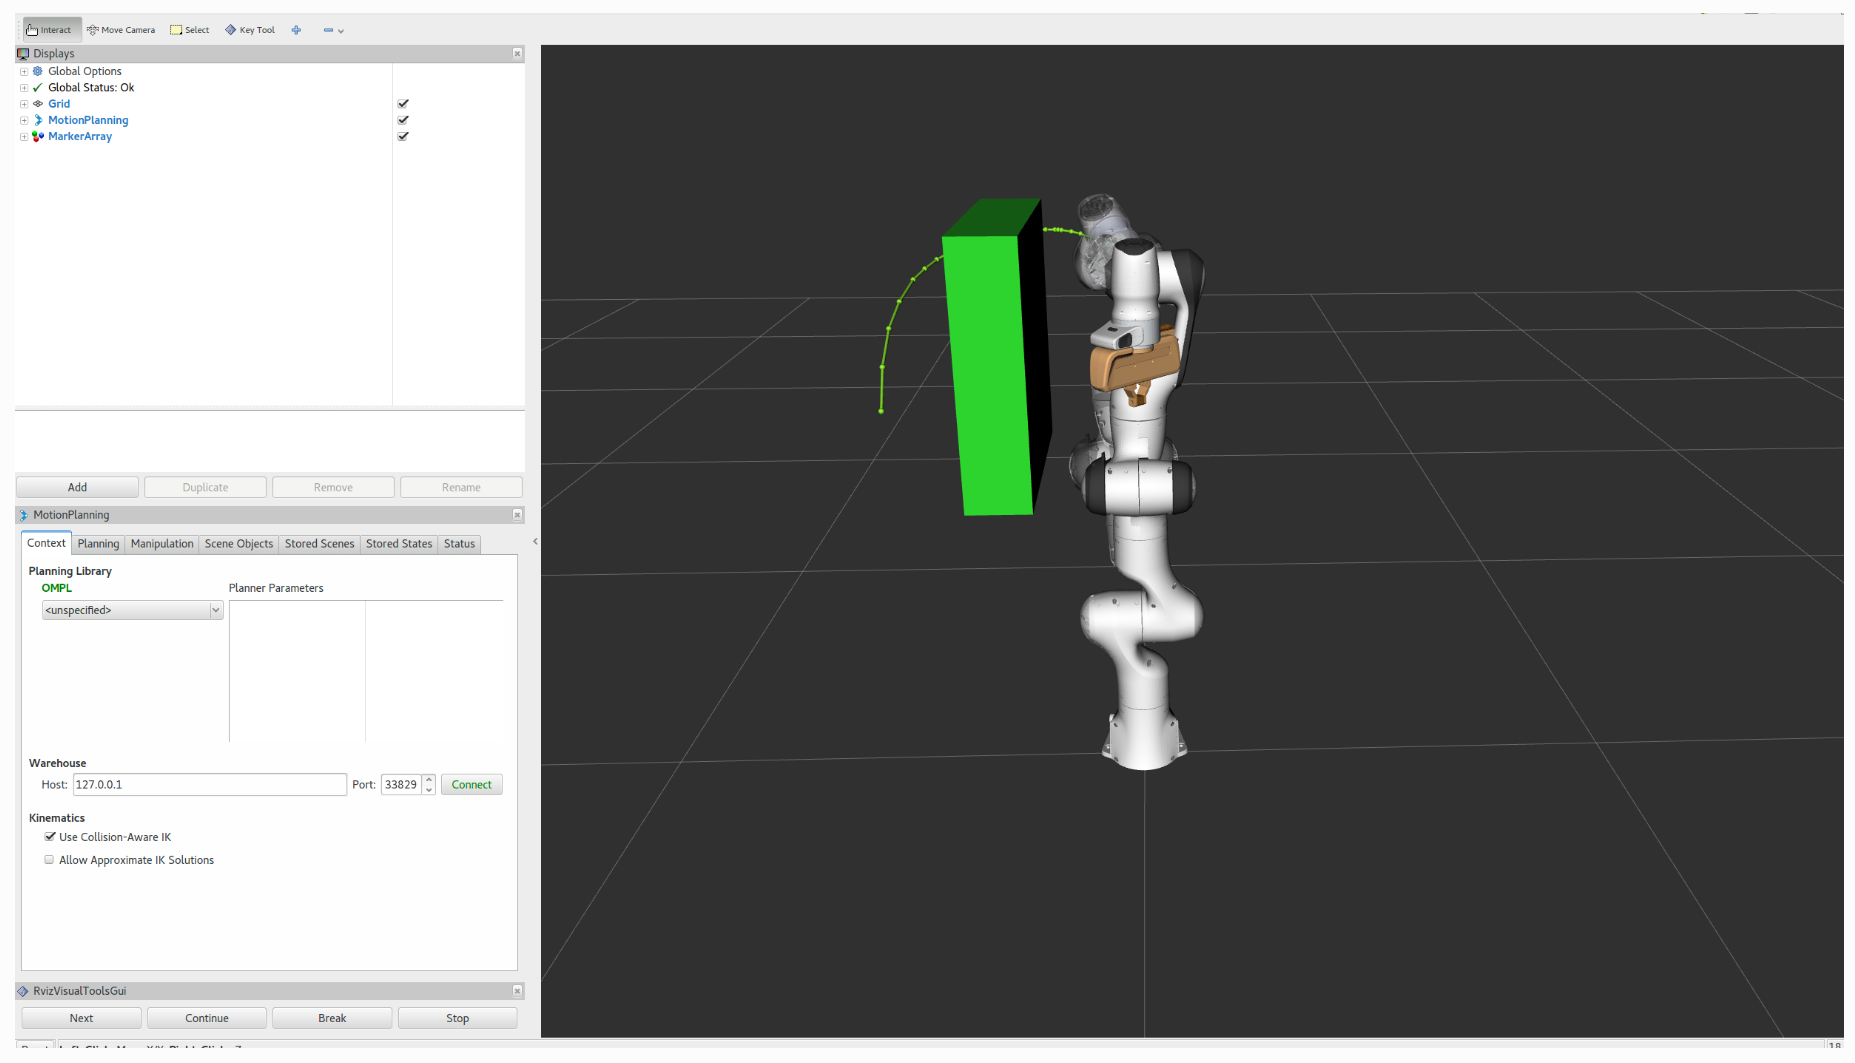
\includegraphics[width=0.95\textwidth]{figures/chapter1-motion-planning}
    \caption{An illustrative path planning task: a manipulator computing a collision-free path around an obstacle.}
    \label{fig:motion-planning-example}
\end{figure}

In practice, this software is central to experimental reproducibility and to the transition from simulation to physical deployment, so qualities such as correctness, reliability, and long-term sustainability have direct consequences for both research and operational outcomes. A simulator that produces incorrect trajectories, or a planner that crashes under realistic inputs, can compromise experimental results.

Software engineers have developed methods and tools for improving software quality: version control, automated testing, and continuous integration are standard practice in professional contexts. However, a gap exists between these practices and what researchers actually do when developing scientific software. Scientists and engineers working on research software tend to learn software engineering skills informally, picking them up from colleagues or through trial and error rather than through formal training~\citep{Hannay2009}. \citet{Hannay2009} observe that many scientists show indifference to standard software engineering concepts, and \citet{Prabhu2011} report that more than half of the scientists they surveyed did not use a debugger. Because much of the software studied in this report originates in research settings, these concerns apply directly to the MPS domain.

Previous studies of the state of the practice have investigated this gap across several scientific software domains, most recently medical imaging~\citep{Smith2024MI} and Lattice Boltzmann method software~\citep{Smith2024LBM}; Section~\ref{sec:state-of-practice-background} reviews these studies. This report adapts the same methodology~\citep{Smith2021} to MPS software. The aim is to understand how MPS software holds up against established software engineering practices and how it compares with other research software domains. The report ranks the selected packages according to the defined quality attributes; these rankings describe the current state of the practice in software development, rather than serving as recommendations for any particular software package.

The remainder of this chapter states the research questions (Section~\ref{sec:research-questions}), defines the scope (Section~\ref{sec:introduction-scope}), overviews the methodology (Section~\ref{sec:methodology-overview}), lists the contributions (Section~\ref{sec:contributions}), and outlines the remaining chapters (Section~\ref{sec:organization}).

\section{Research Questions}
\label{sec:research-questions}

The following research questions guide this report.

\begin{enumerate}[RQ1.]
    \item What software packages are candidates for the study of the state of the practice for MPS software?
    \item What is the ranking of the candidate packages from RQ1 with respect to the software qualities of installability, correctness and verifiability, surface reliability, surface robustness, surface usability, maintainability, reusability, surface understandability, and visibility and transparency?
    \item How do MPS projects compare to other research software domains with respect to the artifacts present in their repositories?
    \item How do MPS projects compare to other research software domains with respect to the use of tools?
    \item How do MPS projects compare to other research software domains with respect to the principles, processes, and methodologies used?
    \item What are the pain points for developers working on MPS software projects?
    \item How do the pain points for MPS developers compare to the pain points for developers in other research software domains?
    \item For MPS developers, what specific best practices address the pain points identified in RQ6 and the software qualities mentioned in RQ2?
    \item What research software development practices, beyond those already used by MPS developers, address the pain points identified in RQ6?
\end{enumerate}

RQ1--RQ5 are answered from public artifacts, while RQ6--RQ9 depend on the developer-interview component.

\section{Scope}
\label{sec:introduction-scope}

This report covers MPS software: robotics packages for motion planning, dynamics, physics, simulation, and supporting middleware. To be included, a package must expose sufficient public evidence, such as a source repository, documentation, issue tracker, releases, or project metadata, to support consistent repository-based measurement. Tools whose core components are proprietary or otherwise closed therefore fall outside the measured set even if they are widely used in robotics practice. Chapter~\ref{ch:methodology} states the full inclusion and exclusion criteria and gives the rationale for individual tools that were considered and removed.

The selected packages play different roles within shared MPS workflows; Chapter~\ref{ch:selected-software-commonality} explains those roles before the measurement results are interpreted.

\section{Overview of the Methodology}
\label{sec:methodology-overview}

This report follows the methodology of \citet{Smith2021} (hereafter the Domain~X methodology): it defines the MPS domain, identifies candidate packages from academic, community-curated, and auxiliary LLM-assisted sources, filters them to a measurable set, measures and ranks the selected packages from their public artifacts, analyzes them as a software family, compares the findings with prior domain studies, and prepares the developer-interview component. Chapter~\ref{ch:methodology} details each step. The scope and exclusions were reviewed with a domain expert to reduce the risk of misrepresenting the MPS domain.

\section{Contributions}
\label{sec:contributions}

This report makes the following contributions:

\begin{enumerate}
    \item A scoped study of the state of the practice for MPS software, applying the methodology of \citet{Smith2021} to a new domain.
    \item A transparent candidate discovery and selection process that combines academic sources, community-curated lists, and auxiliary LLM-assisted discovery, with explicit discussion of the role and limitations of each source type.
    \item A public-artifact measurement dataset for 28 selected software packages, covering repository evidence, documentation, releases, issue trackers, testing and continuous-integration evidence, and project metadata, organized across the nine quality categories defined in the measurement template of \citet{Smith2021}.
    \item A commonality analysis identifying shared capabilities, variability points, and parameters of variation across the selected packages.
    \item A comparison of MPS software with findings from prior studies of the state of the practice in other research software domains~\citep{Smith2024LBM,Smith2024MI,Smith2018Seismology}.
\end{enumerate}

These contributions are descriptive and methodological.

\section{Organization}
\label{sec:organization}

The remainder of this report is organized as follows. The research questions are not confined to a single chapter; they are answered throughout the body, and each chapter notes the research questions it addresses to maintain traceability back to Section~\ref{sec:research-questions}.

\begin{itemize}
    \item \textbf{Chapter~\ref{ch:background}} provides background on the MPS domain, prior studies of the state of the practice, the nine quality attributes, commonality analysis, and the Analytic Hierarchy Process.
    \item \textbf{Chapter~\ref{ch:methodology}} describes the methodology, from domain selection and candidate discovery to measurement, commonality analysis, and the interview component.
    \item \textbf{Chapter~\ref{ch:selected-software-commonality}} presents the 28 selected packages as a software family and reports the commonality analysis.
    \item \textbf{Chapter~\ref{ch:measurement-results}} reports the measurement results, the quality-based rankings, and their comparison with community-facing indicators.
    \item \textbf{Chapter~\ref{ch:comparison-research-software}} compares MPS software with prior studies in other research software domains.
    \item \textbf{Chapter~\ref{ch:developer-interviews}} sets out the developer-interview component for RQ6--RQ9.
    \item \textbf{Chapter~\ref{ch:recommendations}} gives recommendations for future MPS software practice.
    \item \textbf{Chapter~\ref{ch:threats-to-validity}} discusses threats to validity.
    \item \textbf{Chapter~\ref{ch:conclusions}} summarizes the study, answers the research questions, and identifies directions for future work.
\end{itemize}
